\chapter{Descripción del hardware}\label{chp-02}

\lettrine[lraise=-0.1, lines=2, loversize=0.2]{U}na vez conocidas las funciones
que debe desempeñar el sistema es importante definir el hardware a usar para que
sea capaz de cumplimentar los requerimientos establecidos. Los principales dispositivos
utilizados en el proyecto son los siguientes:

\section{Arduino Mega 2560}

Se trata de una placa de desarrollo que cuenta con el microcontrolador ATmega2560 y todo lo
necesario para prototipar un sistema. Cuenta con 54 pines de entrada y salida (GPIO), de los cuales
15 pueden utilizarse como salida PWM, 4 puertos UART, oscilador de 16 MHz, conexión USB tipo B,
pines ICSP de programación y botón de reinicio.

\begin{figure}[hbtp]
	\centering
	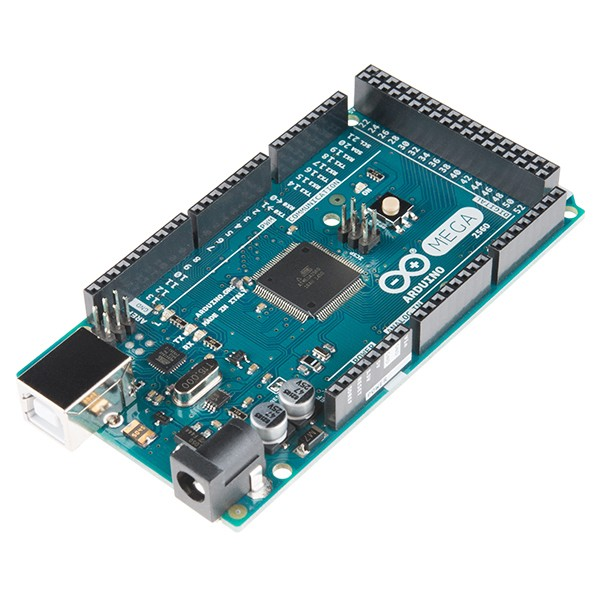
\includegraphics[scale=0.5]{02-hardware/01-arduino-mega-2560.jpg}
	\caption{Arduino Mega 2560}
	\label{fig:figura2}
	\end{figure}


\begin{table}[hbtp]
    \begin{center}
    \begin{tabular}{ | c | c |  }
    \hline
    Microcontrolador & ATmega2560 \\ \hline
    Tensión de funcionamiento & 5 V \\ \hline
    Voltaje de entrada recomendado & 7-12 V \\ \hline
    Voltaje de entrada límite & 6-20 V \\ \hline
    Pines de E/S digitales & 54 (de los cuales 15 con salida PWM) \\ \hline
    Pines de entrada analógica & 16 \\ \hline
    Corriente CC por pin & 20 mA \\ \hline
    Corriente CC para pin 3.3 V & 50 mA \\ \hline
    Memoria Flash & 256 kB, 8 kB utilizados por el gestor de arranque \\ \hline
    SRAM & 8 kB \\ \hline
    EEPROM & 4 kB \\ \hline
    Frecuencia de reloj & 16 MHz \\ \hline
    Longitud & 101.52 mm \\ \hline
    Anchura & 53.3 mm \\ \hline
    Peso & 37 g \\ \hline

    \end{tabular}
    \end{center}
    \caption{Características Arduino Mega 2560}
    \label{tab:tab1}
    \end{table}


\subsection{Alimentación}

El Arduino Mega 2560 puede ser alimentado mediante la conexión USB tipo B proporcionada por
un ordenador o por una fuente de alimentación externa. Además, puede ser alimentado por los pines
de alimentación de la placa, que se describen a continuación:

\begin{itemize}
    \item VIN. Entrada de tensión de la placa cuando hay alimentación externa.
    \item 5V. Pin que produce 5V regulados.
    \item 3V3. Pin que produce 3.3V regulados con un consumo máximo de 50 mA.
    \item GND. Pin de conexión a masa.
    \item IOREF. Referencia de tensión de trabajo del microcontrolador.
\end{itemize}

\subsection{Memoria}

El ATmega2560 cuenta con 256 kB de memoria flash de los cuales 8 kB se usan para el gestor de arranque,
8 kB de memoria SRAM y 4 kB de EEPROM.

\subsection{Entradas y Salidas}

El Arduino Mega cuenta con 54 pines que pueden ser utilizados como salida o entrada digital mediante
las funciones pinMode(), digitalWrite() y digitalRead(). Los niveles lógicos son de 5V. Cada pin soporta
una corriente de 20 mA y cuenta con una resistencia de pull-up de entre 20 y 50 k$\Omega$. Además, algunos pines
tienen funciones especiales:

\begin{itemize}
    \item Comunicación serie. Se usa para recibir y transmitir datos en serie TTL. Son las parejas 0 y 1,
    14 y 15, 16 y 17 y 18 y 19. Los pines 0 y 1 son los correspondientes a la comunicación con el conversor 
    USB-TTL integrado en la placa
    \item Interrupciones externas. Se utilizan para activar interrupciones en el software. Son los pines 2, 3, 18, 19, 20 y 21.
    \item Salida PWM. Proporcionan una salida modulada con 8 bits de precisión con la función analogWrite(). Son los pines del 
    2 al 13 y del 44 al 46.
    \item Comunicación SPI. Pines 50 (MISO), 51 (MOSI), 52 (SCK), 53 (SS). Permiten comunicación SPI con otros 
    dispositivos utilizando la biblioteca SPI.
    \item LED integrado. En el pin 13 hay un LED integrado que puede encenderse con un valor HIGH y apagarse con un valor LOW.
    \item Comunicación TWI. Pines 20 (SDA) y 21 (SCL). Permite comunicación I2C/TWI.
\end{itemize}

\subsection{Comunicación}

La placa Arduino Mega cuenta con diversas formas para comunicarse con un ordenador o con otros dispositivos. El ATmega2560
cuenta con cuatro UART de hardware para comunicación TTL a 5V, una conexión SPI y una conexión I2C. Mediante uno de los puertos
UART el ATmega2560 se comunica con un ATmega16U2 que canaliza la conexión mediante USB a un ordenador y permite la comunicación
entre ambos. Esto permite tanto programar la placa mediante el IDE de Arduino como recibir mediante monitor serie datos simples.

\section{Ethernet Shield de Arduino}

El Ethernet Shield de Arduino se trata de una placa que añade
la funcionalidad de conectar una placa de Arduino a una red 
mediante conexión Ethernet. Se trata de una placa basada en
el chip Wiznet W5100 que provee de una pila de red IP capaz de
soportar protocolos TCP y UDP. Usa la librería Ethernet para leer y 
escribir flujos de datos.

La placa cuenta con varios LED que proporcionan información:
\begin{itemize}
    \item ON. Indica que la placa está alimentada.
    \item LINK. Indica presencia de enlace de red.
    \item 100M. Indica la existencia de conexión de red de 100 Mb/s.
    \item RX. Indica que se reciben datos cuando parpadea.
    \item TX. Indica que se transmiten datos cuando parpadea.
\end{itemize}

Unos puntos importantes del Ethernet Shield son:
\begin{itemize}
    \item Funciona a 5V.
    \item Tiene un microcontrolador W5100 con 16k de buffer y 
    es independiente de la memoria del ATmega2560.
    \item Se comunica con el ATmega2560 mediante SPI.
    \item Soporta 4 conexiones simultáneas.
    \item Utiliza la librería Ethernet.
    \item Dispone de lector de tarjetas microSD para guardar ficheros.
    \item Utiliza los pones 10, 11, 12 y 13 para comunicarse con el
    W5100 mediante SPI.
\end{itemize}

\section{Motor DC y Driver L298N}

El principal actuador de este proyecto es un motor de corriente
continua que es el que mueve la cinta transportadora, permitiéndola
avanzar, retroceder o pararse. Este motor funciona a 24V y tiene 
infinidad de uso, ya que son sencillos de operar y tienen un bajo coste.

Para controlar dicho motor se utiliza un Driver L298N, que está basada
en un puente H. Dicho módulo es capaz de controlar dos motores de 
corriente continua o un motor paso a paso bipolar de hasta 2A.

La principal funcionalidad del módulo es separar la parte asociada
a la potencia (que funciona a 24V en este caso) de la parte asociada
al control (que funciona a 5V).

\subsection{Conexionado del módulo L298N}

El módulo cuenta con un circuito integrado LM7805 que proporciona 5V
que puede ser activado o desactivado mediante un jumper.

Mientras el jumper esté activo, la placa admite tensiones de 
alimentación de entre 6 y 12V. Así, la conexión de 5V será una salida.

Por otra parte, si el jumper está desactivado la placa admite tensiones
de alimentación de entre 12 y 35V. En este caso se deberá proporcionar
5V de referencia a la placa para el funcionamiento de la parte lógica.

\section{Encoder Rotativo Incremental}

Para posicionar correctamente las piezas a lo largo de la cinta es
necesario contabilizar el movimiento de la misma. Para ello, se cuenta
con un encoder rotativo incremental de serie LPD3806-600BM el cual
cuenta con una gran precisión.

Éste tiene dos salidas de onda cuadrada con un desfase de 90 grados
entre ellas. 


\subsection{Especificaciones técnicas}

El encoder rotativo de serie LPD3806-600BM cuenta con las
siguientes especificaciones:
\begin{itemize}
    \item 600 pulsos/revolución por cada fase. Por lo tanto, con las
    fases combinadas se cuenta con 2400 pulsos/revolución.
    \item Velocidad máxima: 5000 revoluciones/minuto.
    \item Respuesta de frecuencia: 0-30KHz
\end{itemize}

\subsection{Conexionado del Encoder}

El encoder cuenta con cuatro cuables de conexión:
\begin{itemize}
    \item Rojo. Alimentación 5-24V.
    \item Negro. GND.
    \item Verde. Fase A.
    \item Blanco. Fase B.
\end{itemize}

\section{Calibrador digital}

\section{LCD}

\section{Sensor fotoeléctrico OMRON}

\section{Banda transportadora con elementos integrados}

\section{Controlador IRC5C}